\chapter{Power System Overview}
As discussed in the introduction, the modeled electrical power system is a 40
kWe, recuperated Brayton cycle driven by a direct-cooled nuclear fission reactor. The goal
of the project was to develop a mass model for the major components of the
electrical power system. These mass models were then used to explore the
tradeoff in performance and mass between each of the systems. In general terms,
an efficient power conversion cycle requires a smaller thermal input, but is
more massive. Conversely, a less massive power cycle has lower efficiency,
requiring a larger thermal input. This section will provide context to the
development of the reactor mass model.

\section{Cycle Description and Mass Modeling}
The modeled cycle was a direct Brayton cycle coupled to a fission reactor. The
cycle was recuperated for increased efficiency. A cycle diagram is shown below
with the three modeled components. Figure \ref{fig:power_cycle} shows the power
cycle diagram for this system.

\begin{figure}[h]
    \centering
    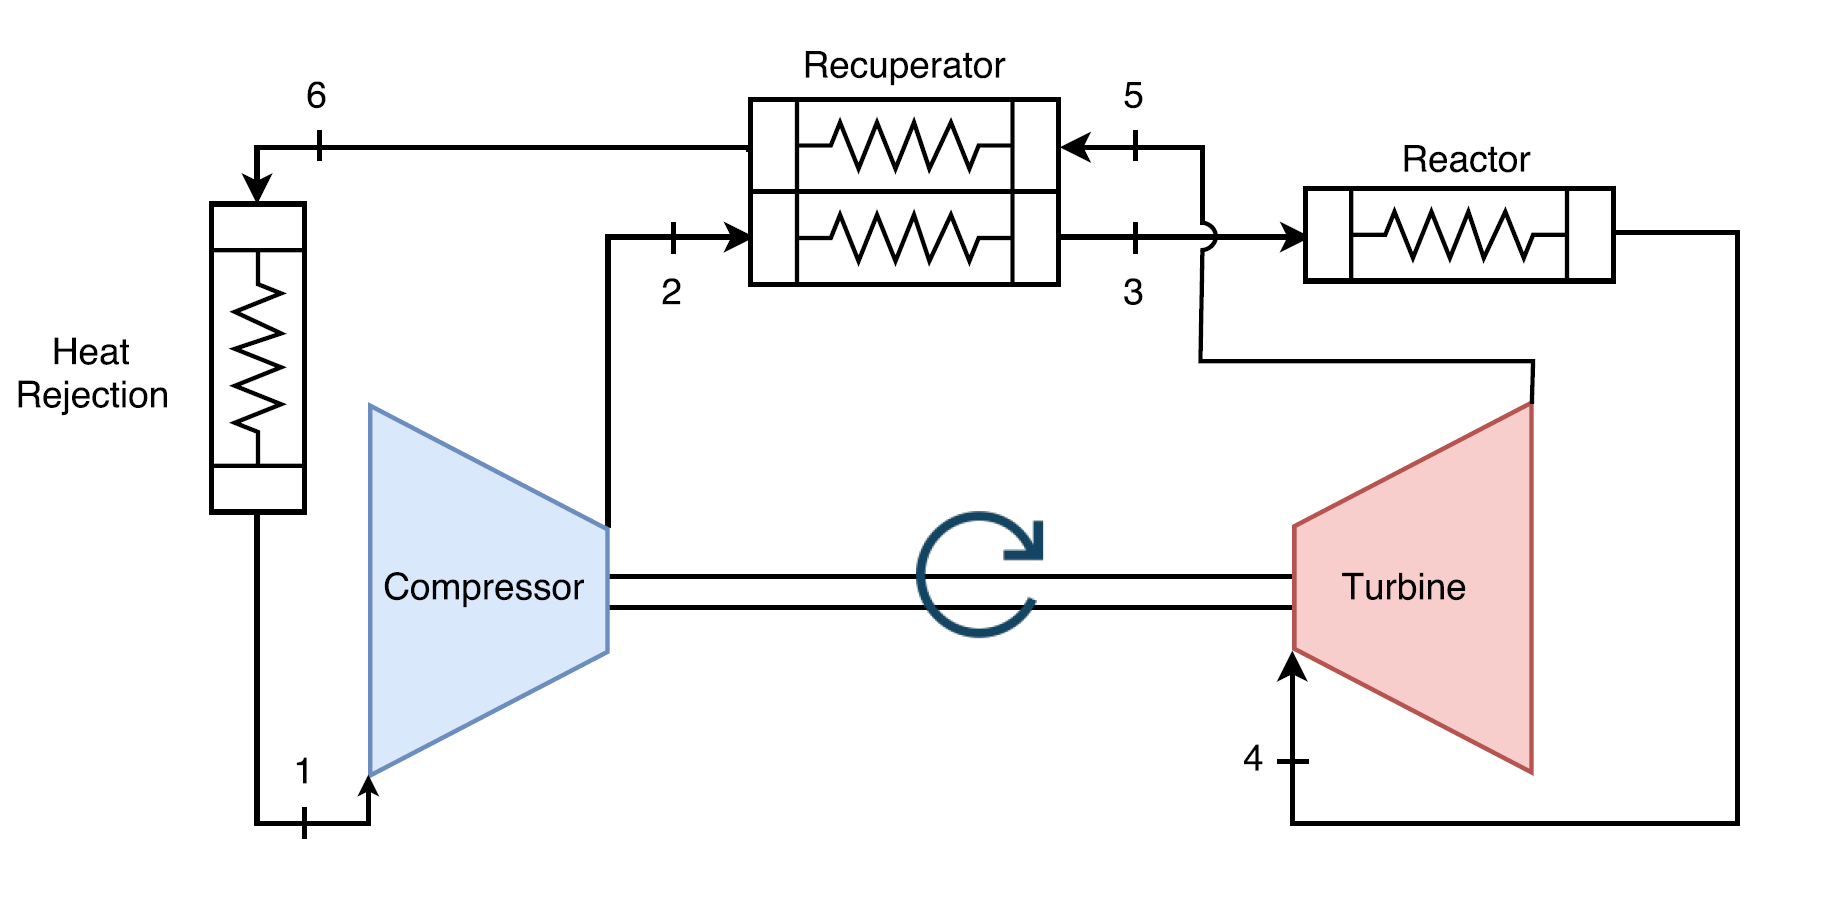
\includegraphics[width=5in]{../images/power_cycle.png}
\caption{Power cycle diagram}
\label{fig:power_cycle}
\end{figure}

Three main power system components were modeled for
mass; the radiator, recuperator, and the reactor. This thesis focuses on the
reactor mass model. The goal of this work was to deliver a mass
model to a colleague in order to optimize the overall power cycle mass
performance. The colleage developed mass models for the radiator and recuperator
as well as a cycle model to model the thermodynamic performance of the system.
Turbine and compressor masses were not modeled, these were off-the-shelf
components. Even if the compressor and turbine were custom-designed, their
negligible mass contribution to the power cycle mass would make optimizing their
design relatively fruitless.

\subsection{Reactor Coupling}
The interface between the reactor and the rest of the power cycle were flow
conditions. The reactor thermal output was determined by the required enthalpy
input to match the power cycle performance and meet the 40 kWe project
requirement. The flow conditions were important for two reasons, they dictated
the thermal power requirements for the core, and they impacted the convective
heat transfer from the reactor cladding to the coolant. The flow properties
provided by the power cycle model were:

\begin{enumerate}
    \item inlet/outlet temperature
    \item inlet/outlet pressure
    \item mass flow rate
    \item thermal power
\end{enumerate}

These conditions were taken as inputs to the power cycle model. For the sake of
cycle optimization, the model returned a reactor mass that matched the flow
conditions and thermal power requirements. For future neutronics modeling, the
model could also return geometric core parameters (radius, fuel fraction,
reflector thickness, etc.). 

\section{Initial Reactor Design Constraints}
    In order to develop a reactor mass model, the concept was constrained with
some general design decisions. The chosen design needed to be simple and robust. The simplest reactor fuel concept is block fuel with coolant channels. 
Block fuel is a common design choice for space reactors that operate at relatively 
low power and burnup compared to power reactors. Two fuel types were chosen; one for
near-term and the other for long-term technological readiness options. Uranium
oxide was chosen as the near-term fuel option for its high melting temperature.
UMo and UN fuel were not considered because of tempearture limitations, despite
their thermal conductivity and uranium density advantages. Inconel-718 was
chosen as cladding for its high temperature strength and corrosion
compatability with sCO$_2$. With these design choices, the reactor mass model
could be developed from first principle heat transfer and fluid flow equations
coupled with a critical core radius constraint.

\subsection{Fuel Composition}
Two reactor fuels were considered for modeling. The near term technical
readiness choice was 93\% enriched \uox. The advanced fuel option investigated
was 93\% enriched uranium-tungsten cermet (UW). UW-cermet fuel is UN fuel suspended in a
tungsten matrix. UW-cermet fuel has been considered for nuclear thermal
propulsion due to its high thermal conductivity and resistance to fuel swelling.
The tradeoff with UW-cermet fuel is a reduced uranium density, 60\% of the fuel
volume is UN, 40\% is tungsten. As shown below in Table \ref{tab:uox_comp} and
Table \ref{tab:uw_comp}, the \uox fuel has a significantly higher uranium
density than the UW-CERMET fuel.

\begin{table}[h]
  \centering
  \caption{\uox fuel composition}
  \begin{tabular}{cc}
    \toprule
    Isotope   & Mass Fraction [-] \\
    \midrule
     8016     & 0.1520 \\
    92235     & 0.7886 \\
    92238     & 0.0594 \\
  \end{tabular}
  \label{tab:uox_comp}
\end{table}
    
\begin{table}[h]
  \centering
  \caption{UW-CERMET fuel composition}
  \begin{tabular}{cc}
    \toprule
    Isotope   & Mass Fraction [-] \\
    \midrule
     7015     &  0.0260 \\
     74180    &  0.0006 \\ 
     74182    &  0.1396 \\
     74183    &  0.0758 \\
     74184    &  0.1632 \\
     74186    &  0.1531 \\
     92235    &  0.4107 \\
     92238    &  0.0309 \\
  \end{tabular}
  \label{tab:uw_comp}
\end{table}

\newpage

\subsection{Fuel Design Modularity}
A fuel design was chosen to constrain the reactor model. In order to support
alternate designs, the reactor model was developed in a modular fashion.
Different fuel configurations such as pin-type or TRISO particle fuel could be
explored with a different set of heat transfer equations and criticality models.
This will be discussed in more detail in following sections.


\section{Model Development}
The reactor and power cycle models were developed independently and combined
near the end of the project to model the entire system. While the reactor model
was under development, a simplified analytic model was used in place of the
reactor model to return an estimate of reactor mass. While the power cycle model
was under development (in tandem with the reactor model), a set of assumed flow
inputs were used to simulate a power cycle thermal load. The reactor model was
developed in Python and the power cycle model was developed in MATLAB. This
unintentional mismatch in development choices proved interesting when it came
time to merge the models! Despite this challenge, the reactor model was smoothly
imported into the MATLAB power cycle model and the two models worked seamlessly
to model the overall cycle mass.
